\section{Overview}
\label{oram:overview}
Consider a database with $N$ blocks of data shared among $c$ clients.
\sysname~ stores the data blocks in a RingORAM on the server and the position map entries for the RingORAM in a server hosted 
pyramid ORAM (PD-ORAM). 
The stash for the RingORAM (which 
holds blocks that overflow from the RingORAM tree) is also stored on the server. 
Since, the stash can grow (and shrink) dynamically after an eviction, this allows the server to learn 
the number of blocks that have been evicted to the tree during a RingORAM eviction. To prevent this leak, \sysname~ 
allocates a fixed sized stash which is equal to the maximum size that the stash can grow as determined by the experimental 
upper bound in \cite{ringoram}.

{\bf Position map.~}
%
Each position map entry is indexed by a logical block ID and contains 
the corresponding leaf ID in the RingORAM tree to which that data block is mapped, or 
indicates that the block is in the stash. Since each level of PD-ORAM contains multiple fixed-sized buckets, 
an entry for a particular logical block ID, if it exists in a PD-ORAM level, is located 
in the bucket determined by applying the secret hash function for that level on the 
logical block ID. Clients query for a position map item by downloading the corresponding buckets
from each level of PD-ORAM as determined by the hash function for that level. 
Further, the top level of PD-ORAM is designed to contain as many entries as the size of the stash. 
This ensures that during an eviction, even if the entire stash is evicted to the tree, the entries for these 
blocks can be added to the top level of PD-ORAM.

In addition, the server maintains 
three append-only logs: query log, position map (PM) result log 
and data result log. The logs are stored encrypted on the server.


{\bf Query log.~}
%
The query log records all currently ongoing transactions. Clients 
append the logical ID of the data block they are querying for and download
the query log to check for overlapping accesses. 
In the case where the required data block is already being accessed by another client (and there 
is a previous entry in the query log for the same), the client 
proceeds with a dummy access (described later). The query log ensures that all 
clients have a consistent view of ongoing transactions and thus do not query for the 
same block.

{\bf PM result log.~}
%
The PM result log contains items that have been accessed from the position map 
in the last round of concurrent accesses. After reading an entry from the 
position map, a client reencrypts and return the entry to the server which is appended to the PM 
result log. 

{\bf Data result log.~}
%
The data result log contains the data blocks that have been accessed from the 
RingORAM in the last round of concurrent accesses. After finding the required block from either 
the requested path in the RingORAM tree or the stash, 
a client reencrypts and return the item to the server which is appended to the data 
result log.


\begin{figure}
 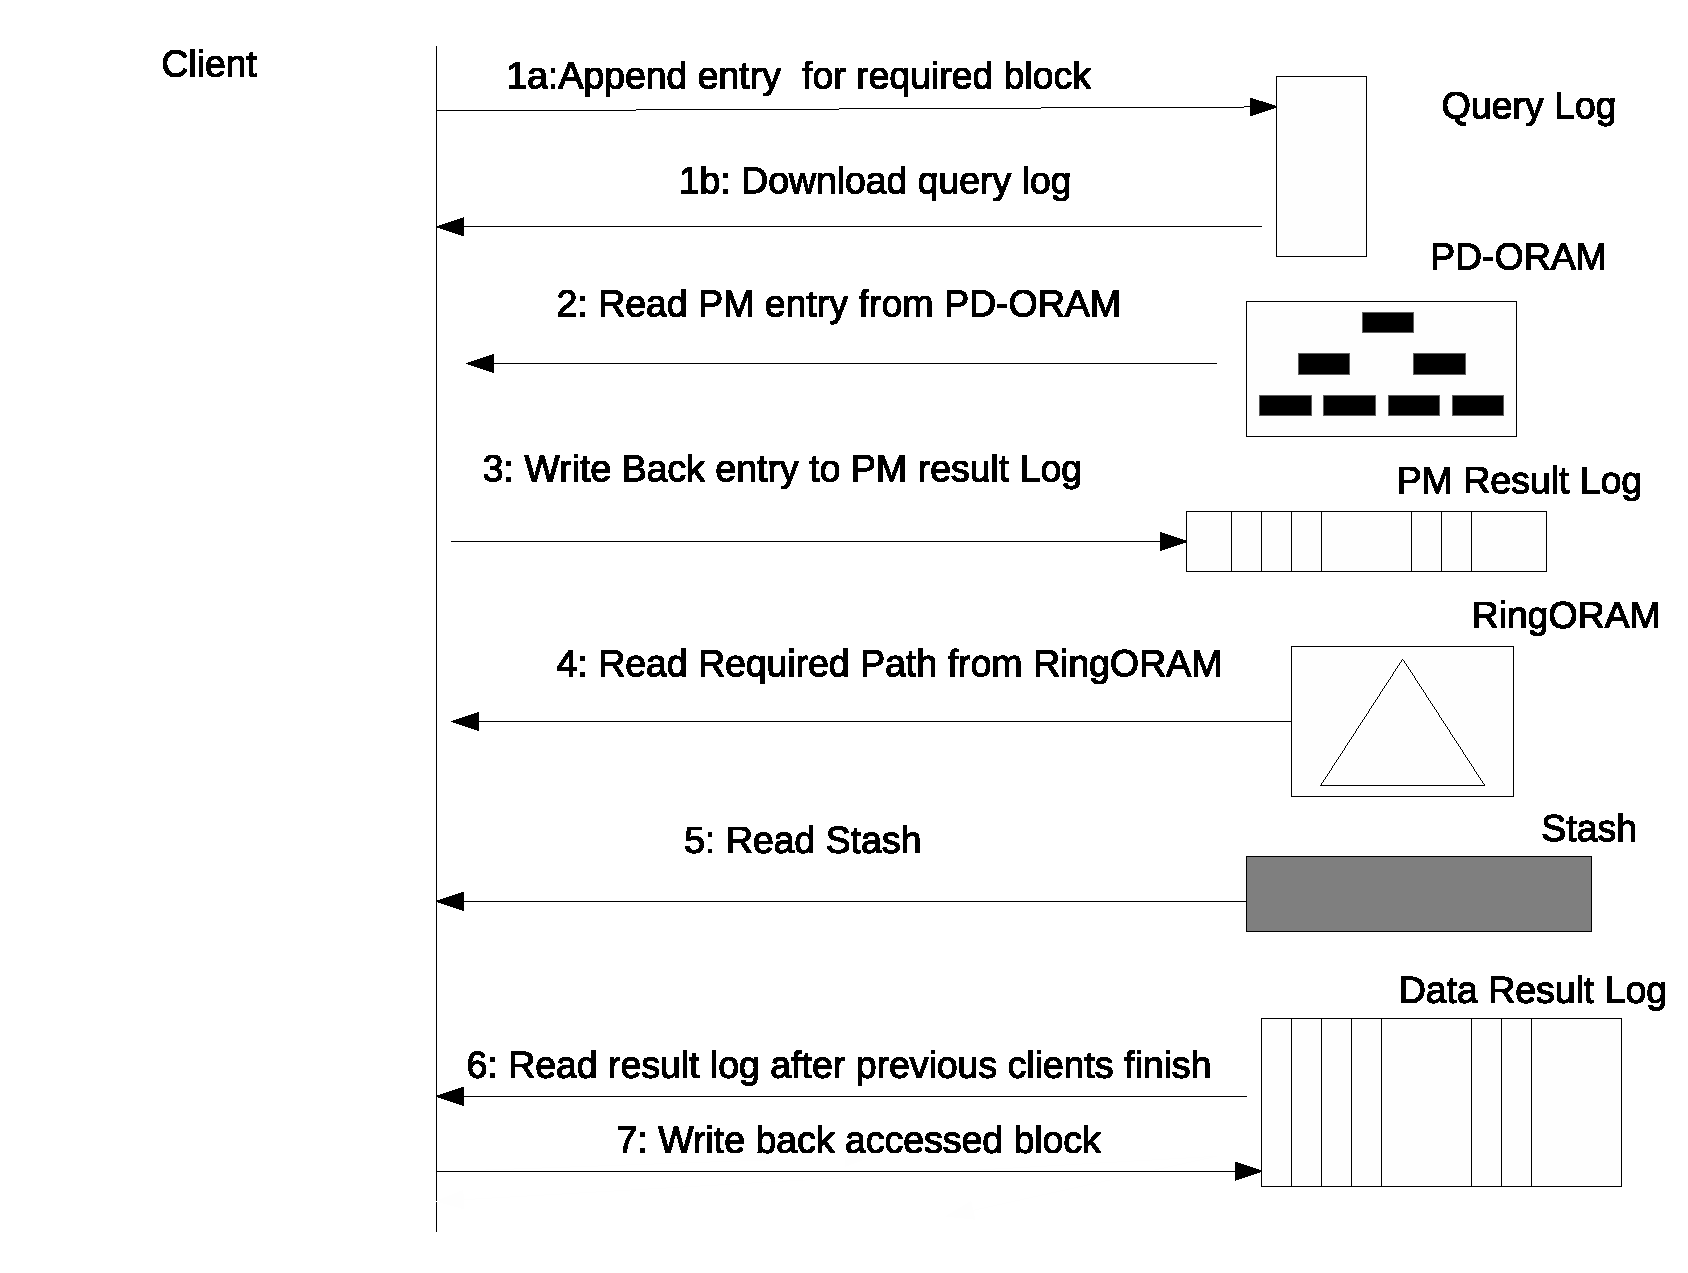
\includegraphics[scale=0.30]{Figures/Query_overview.eps}
 \caption{Overview of a query. Steps 1-6 can proceed concurrently. In step 7, clients wait for previous clients to finish before downloading
 data result log \label{query_overview}}
\end{figure}


Figure \ref{query_overview} shows the query protocol for \sysname~. Queries proceed as follows: 
\begin{enumerate}
 \item In step 1a and step 1b, a client appends the logical block ID of the required block and downloads the query log. If the required block 
 is already being accessed, the client proceeds with a dummy access in the following steps.
 \item In step 2, the client reads a bucket from each level of PD-ORAM to locate the position map entry for the required logical block ID. The PD-ORAM access protocol 
 ensures that the client finds the required position map entry in this step. For a dummy access, the client reads a random bucket from each level of PD-ORAM.
 \item In step 3, the client reencrypts and writes back the actual position map entry read in Step 2 to the PM result log. For a dummy access, the client writes a ``fake'' 
 item to the PM result log (such as an encryption of all zeroes).
 \item In step 4 and 5, the client reads a block from each bucket on the RingORAM path 
 on which the queried block exists (as determined from the position map entry) and the stash. For a dummy access, 
 the client reads dummy blocks from a randomly selected path.
 \item In step 6, the client reads the data result log after all previous clients finish. If a client has executed 
 a dummy query, the client gets the required block from the data result log. 
 \item If a client found the required block in step 6, the client writes back the updated value of the block to the 
 data result log for a write access. Otherwise, the client reencrypts and writes back the accessed block.
\end{enumerate}

Note that in step 7, a client finds the most updated version of the 
required block after all previous ongoing transactions accessing the block has completed. 

\begin{figure}
 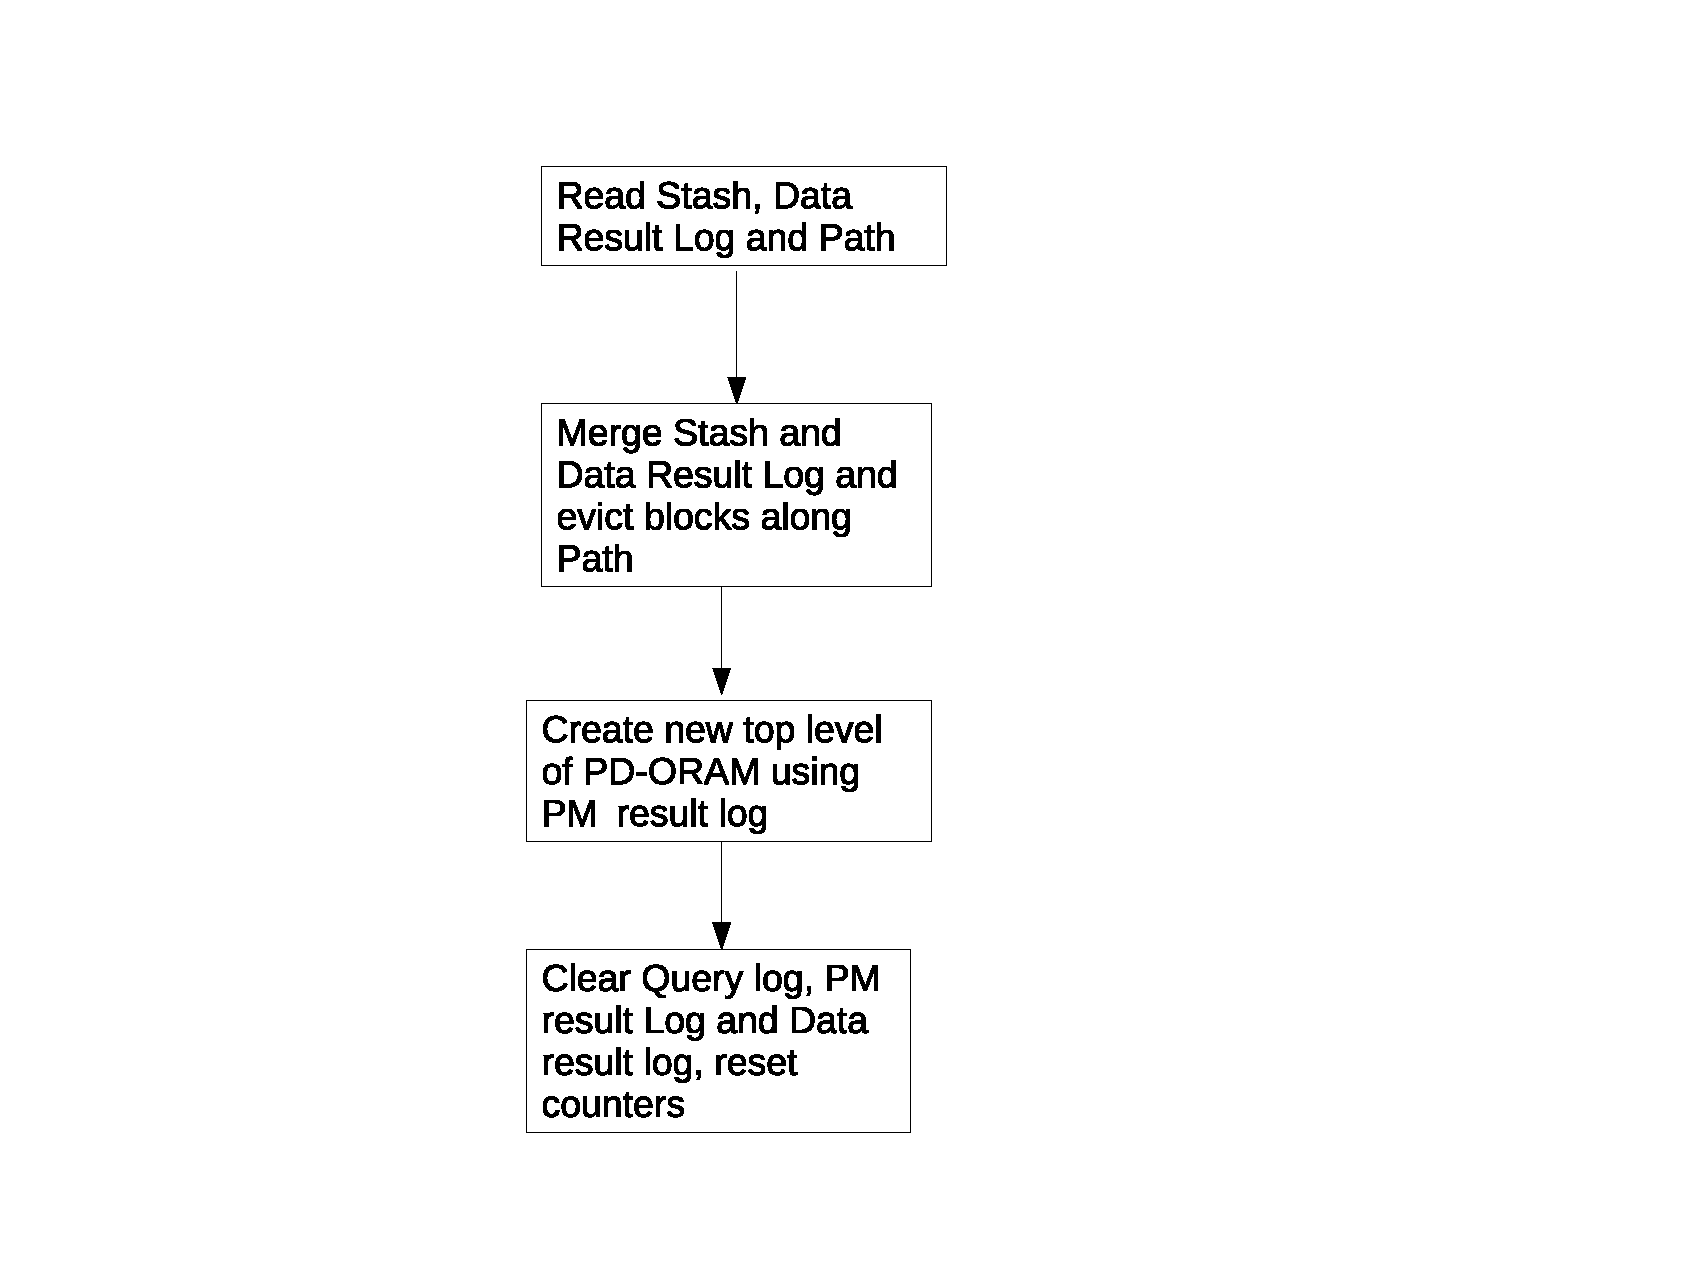
\includegraphics[scale=0.30]{Figures/eviction.eps}
 \vspace{-1cm}
 \caption{High level description of the eviction process. The path to be evicted is chosen in the reverse lexicographical order. \label{eviction_fig}}
\end{figure}


{\bf Eviction.~}
After a fixed number of accesses, the logs are cleared through an eviction to the 
RingORAM tree (Figure \ref{eviction_fig}). 
More specifically, after $k$ (a fixed parameter) concurrent queries,  
the client with the last query reads the logs, the stash and a predetermined path 
from the RingORAM tree (chosen in the reverse lexicographical order) 
and tries to evict blocks in the data result log and the stash 
to the path. First, the data result log and the stash are merged. 
Since, there may be multiple compies of the same block in the data result log due to concurrent accesses for the same 
block, only the latest copy of a block in the data result log is merged with the stash. The client tries to 
evict as many blocks from the stash and data result log combined to the path.
The overflow from the eviction forms the new stash. 

Then, the client creates the new top level 
of PD-ORAM with the new mappings for the evicted blocks. Since, the top level is of fixed size and 
the number of blocks evicted is variable, the client adds ``fake'' entries to ensure that the new top level is 
of the same size irrespective of the outcome of the eviction.  This is similar to Privatefs \cite{privatefs}, 
where the result log becomes the top level of PD-ORAM after a fixed number of accesses. Further, all the logs are cleared after the eviction.

The server maintains an access counter and ensures that the eviction takes place after a fixed number of concurrent accesses. During the eviction, 
the server locks all client accesses to ensure consistency. Note that only in step 7 of the query protocol, clients need to wait for previous clients to 
finish. Moreover, since client queries proceed concurrently, the queries are expected to finish at almost similar times. 



